% ***********************************************************
% ******************* PHYSICS HEADER ************************
% ***********************************************************
% Version 2 
\documentclass[
	12pt,						% Schriftgr��e
	DIV10,						% Druckbaren Bereich variieren
% 	BCOR=1cm,  					% Korrigiert den linken Rand für Buchbindungen
%	headsepline,					% Kopfzeile wird durch Linie abgetrennt
%	smallheadings,					% kleinere Überschriften
	a4paper,					% Papierformat
%	headinclude,
 	oneside,					% einseitiges Dokument
% 	titlepage,					% es wird eine Titelseite verwendet
% 	halfparskip,					% Abstand zwischen Abs�tzen (halbe Zeile)
% 	normalheadings,					% Gr��e der �berschriften verkleinern
% 	liststotoc,					% Verzeichnisse im Inhaltsverzeichnis auff�hren
% 	bibtotoc,					% Literaturverzeichnis im Inhaltsverzeichnis auff�hren
% 	idxtotoc,					% Index im Inhaltsverzeichnis auff�hren
%	draft						% Status des Dokuments (final/draft)
]{scrartcl}
\pagestyle{plain} % mit Parameter headings werden Überschriften in die Kopfzeile eingetragen
% \usepackage[
% 	automark,			% Kapitelangaben in Kopfzeile automatisch erstellen
% 	headsepline,			% Trennlinie unter Kopfzeile
% 	ilines				% Trennlinie linksb�ndig ausrichten
% ]{scrbook}

% Sprach- und Zeicheneinstellungen
\usepackage{color}
\usepackage[utf8]{inputenc} % utf8 ist die latin9 Variante für Linux und ermöglicht Umlaute, Sonderzeichen, etc.
\usepackage[T1]{fontenc} % Typ 1 Schriftart verwendet Umlaute
\usepackage[english]{babel} % Übersetzt automatische Bezeichnungen wie, "chapter"...
\usepackage{lmodern} % weichere Zeichen bei PDFs
%\parindent0pt % kein Einschub bei neuem Paragraph
\usepackage{microtype} % komprimiert die Zeichen- und Wortsetzung und vermeidet damit overfull (underfull) Fehlermeldungen

% Graphiken einbinden
%\usepackage[final]{pdfpages} % pdf files einbinden
\usepackage[final]{graphicx}
\usepackage{float}
\usepackage{caption} % ermöglicht Bildunterschriften zu optimieren, zB. durch
\captionsetup{format=plain}
\usepackage{rotating} % Bilder drehen
%\usepackage{sidecap} % Bildunterschrift neben das Bild setzen
\usepackage{subcaption} % Bildunterschriften unter mehrere Bilder und innerhalb einer figure-Umgebung setzen
%\usepackage{wrapfig}

% Zusätzliches
%\usepackage{fancybox} % \fbox: \shad­ow­box, \dou­ble­box, \oval­box, \Oval­box
\usepackage{multicol} % Allows for multiple columns
\usepackage{color}
\definecolor{black}{gray}{0} % 10% gray
\usepackage{lscape}
\usepackage{pdfpages}
\usepackage[draft=false,colorlinks=true,linkcolor=black,citecolor=black]{hyperref} % ermöglicht von der Referenz zum Label zu 
%springen
%\usepackage{longtable} % Tabellen über mehrere Seiten erstellen
%\usepackage{booktabs} % entzerrt Tabellenzeilen

% Latex-Zeichnungen und Einstellungen
\usepackage{tikz}
\usetikzlibrary{arrows,positioning,fadings,shadows,shadows.blur}
\tikzfading[name=fade out, inner color=transparent!0,
  outer color=transparent!100]
\tikzset{
    %Define standard arrow tip
    >=stealth',
    font=\sffamily\small,
    %Define style for boxes
    rechteck/.style={
           rectangle,
           rounded corners,
           draw=black, very thick,
           text width=6.5em,
           minimum height=2em,
           text centered},
    % Define arrow style
    pil/.style={
	   ->,
	   auto,
	   >=stealth',
	   shorten >=1pt,
           thick},
    % Define standard node style
    main node/.style={circle,fill=blue!15,draw=black,thick,minimum size=6mm,blur shadow={shadow blur steps=5}},
    simple/.style={circle,fill=white!15,draw=black,thick,minimum size=8mm},
    passive/.style={circle,fill=white!15,draw=black,thick,minimum size=6mm,blur shadow={shadow blur steps=5}},
    passiveN/.style={circle,fill=white!15,draw=black,thick,minimum size=8mm,blur shadow={shadow blur steps=5}},
    activeN/.style={circle,fill=red!15,draw=black,thick,minimum size=8mm,blur shadow={shadow blur steps=5}},
    scheme/.style={ellipse,fill=red!15,draw=black,thick,minimum size=8mm,blur shadow={shadow blur steps=5}}
}

% Mathepacket
\usepackage{amsmath} 						% AMS Math Package
\usepackage{amsthm} 						% Theorem Formatting
\usepackage{amssymb} 						% Math symbols such as \mathbb
\usepackage{bbold}
% Mathematische Umgebung definieren zB. \begin{theorem} ...
\newtheorem{theorem}{Theorem}[section]
\newtheorem{lemma}[theorem]{Lemma}
\newtheorem{proposition}[theorem]{Proposition}
\newtheorem{corollary}[theorem]{Corollary}
\newenvironment{definition}[1][Definition]{\begin{trivlist}
\item[\hskip \labelsep {\bfseries #1}]}{\end{trivlist}}
\newenvironment{example}[1][Example]{\begin{trivlist}
\item[\hskip \labelsep {\bfseries #1}]}{\end{trivlist}}
\newenvironment{remark}[1][Remark]{\begin{trivlist}
\item[\hskip \labelsep {\bfseries #1}]}{\end{trivlist}}
% alternative Darstellung mit mdframed
\usepackage[framemethod=TikZ]{mdframed}						% Theorem formatting with a box
\newmdtheoremenv[
  skipabove		=	10pt,
  skipbelow		=	10pt,
  linewidth		=	1pt,
  roundcorner		=	10pt,
  backgroundcolor	=	blue!5,
  innertopmargin	=	10pt,
  innerbottommargin	=	10pt,
  linecolor		=	black,
]{mddef}{Definition}[section]
% include programming script in python 
%\usepackage{listings}
%\lstset{language=Pascal}
%\usepackage{verbatimfiles}


% Anweisungen umbenennen -----------------------------------------------------------------------------------------------------
\makeatletter % Need for anything that contains an @ command 
\renewcommand{\maketitle} % Redefine maketitle to conserve space
{ \begingroup \vskip 10pt \begin{center} \large {\bf \@title}
	\vskip 10pt \large \@author \hskip 20pt \@date \end{center}
  \vskip 10pt \endgroup \setcounter{footnote}{0} }
\makeatother % End of region containing @ commands
\renewcommand{\labelenumi}{(\alph{enumi})} % Use letters for enumerate
% \DeclareMathOperator{\Sample}{Sample}
\let\vaccent=\v % rename builtin command \v{} to \vaccent{}
\renewcommand{\v}[1]{\ensuremath{\mathbf{#1}}} % for vectors
\newcommand{\gv}[1]{\ensuremath{\mbox{\boldmath$ #1 $}}} 
% for vectors of Greek letters
\newcommand{\uv}[1]{\ensuremath{\mathbf{\hat{#1}}}} % for unit vector
\newcommand{\abs}[1]{\left| #1 \right|} % for absolute value
\newcommand{\avg}[1]{\left< #1 \right>} % for average
\let\underdot=\d % rename builtin command \d{} to \underdot{}
\renewcommand{\d}[2]{\frac{d #1}{d #2}} % for derivatives
\newcommand{\dd}[2]{\frac{d^2 #1}{d #2^2}} % for double derivatives
\newcommand{\pd}[2]{\frac{\partial #1}{\partial #2}} 
% for partial derivatives
\newcommand{\pdd}[2]{\frac{\partial^2 #1}{\partial #2^2}} 
% for double partial derivatives
\newcommand{\pdc}[3]{\left( \frac{\partial #1}{\partial #2}
 \right)_{#3}} % for thermodynamic partial derivatives
\newcommand{\ket}[1]{\left| #1 \right>} % for Dirac bras
\newcommand{\bra}[1]{\left< #1 \right|} % for Dirac kets
\newcommand{\braket}[2]{\left< #1 \vphantom{#2} \right|
 \left. #2 \vphantom{#1} \right>} % for Dirac brackets
\newcommand{\matrixel}[3]{\left< #1 \vphantom{#2#3} \right|
 #2 \left| #3 \vphantom{#1#2} \right>} % for Dirac matrix elements
\newcommand{\grad}[1]{\gv{\nabla} #1} % for gradient
\let\divsymb=\div % rename builtin command \div to \divsymb
\renewcommand{\div}[1]{\gv{\nabla} \cdot #1} % for divergence
\newcommand{\curl}[1]{\gv{\nabla} \times #1} % for curl
\let\baraccent=\= % rename builtin command \= to \baraccent
\renewcommand{\=}[1]{\stackrel{#1}{=}} % for putting numbers above =

%---------------------------- TIKZ Bilder -------------------------------------------------------------------------------------

\def\RuleOne{
\begin{tikzpicture}
 \matrix (m) [matrix of nodes,ampersand replacement=\&, column sep=13mm, row sep=1mm]
  {
  \node (1) [activeN ] {}; 		\& 	\node (4) [activeN] {}; \\
  \node (2) {}; 			\&	\node (5) {};		\\
  \node (3) [passiveN] {};		\& 	\node (6) [activeN] {};	\\
  };
  \draw			(1) -- (3);
  \draw		 	(4) -- (6);
  \draw[pil, shorten >=5pt, shorten <=5pt]		(2) -- (5);
\end{tikzpicture}
}

%-----------------------------------------------------------------------------------------------------------------------------

\def\RuleTwo{
\begin{tikzpicture}
 \matrix (m) [matrix of nodes,ampersand replacement=\&, column sep=13mm, row sep=1mm]
  {
  \node (1) [activeN ] {}; 		\& 	\node (4) [activeN, fill=green!15] {};\\
  };
  \draw[pil, shorten >=5pt, shorten <=5pt]	(1) edge node {$N$} (4);
\end{tikzpicture}
}

%----------------------------------------------------------------------------------------------------------------------------

\def\RuleThree{
\begin{tikzpicture}
 \matrix (m) [matrix of nodes,ampersand replacement=\&, column sep=13mm, row sep=1mm]
  {
  \node (1) [activeN ] {}; 		\& 	\node (4) [passiveN ] {};\\
  };
  \draw[pil, shorten >=5pt, shorten <=5pt]	(1) edge node {$N$} (4);
\end{tikzpicture}
}

%-----------------------------------------------------------------------------------------------------------------------------

\def\bspEins{
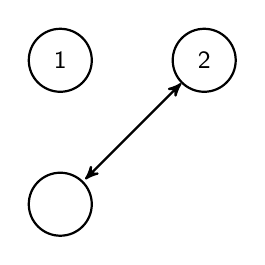
\begin{tikzpicture}[pil]
  \node[simple] (a1) {1};
  \node[simple] (a2) [right=of a1] {2};
  \node[simple] (a3) [below=of a1] {};
  \path[<->]
    (a2) edge (a3);
\end{tikzpicture}
}
\def\bspZwei{
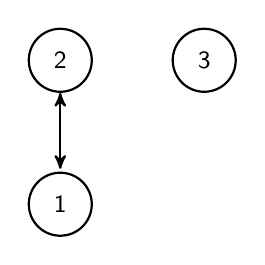
\begin{tikzpicture}[pil]
  \node[simple] (a1) {2};
  \node[simple] (a2) [right=of a1] {3};
  \node[simple] (a3) [below=of a1] {1};
  \path[<->]
    (a1) edge (a3);
\end{tikzpicture}
}
\def\bspDrei{
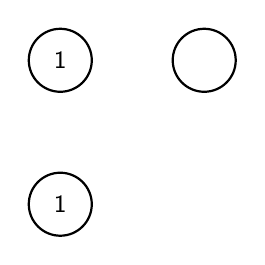
\begin{tikzpicture}[pil]
  \node[simple] (a1) {1};
  \node[simple] (a2) [right=of a1] {};
  \node[simple] (a3) [below=of a1] {1};
\end{tikzpicture}
}
%------------------------------------------------------------------------------------------------------------------------
\def\SingleOutbreak{
\begin{multicols}{5}
\setlength{\columnseprule}{0.4pt}
\centering
t = 1\\[10pt]
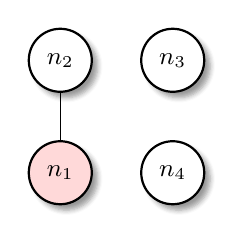
\begin{tikzpicture}[node distance=0.6cm]
  \node[activeN ] (a1) {$n_1$};
  \node[passiveN] (a2) [above=of a1] {$n_2$};
  \node[passiveN] (a3) [right=of a2] {$n_3$};
  \node[passiveN] (a4) [below=of a3] {$n_4$};
  \path
    (a1) edge (a2);
\end{tikzpicture}
\columnbreak

t = 2\\[10pt]
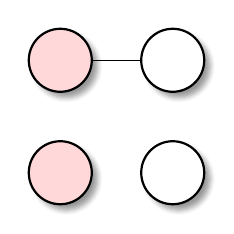
\begin{tikzpicture}[node distance=0.6cm]
  \node[activeN ] (a1) {};
  \node[activeN ] (a2) [above=of a1] {};
  \node[passiveN] (a3) [right=of a2] {};
  \node[passiveN] (a4) [below=of a3] {};
  \path
    (a2) edge (a3);
\end{tikzpicture}
\columnbreak

t = 3\\[10pt]
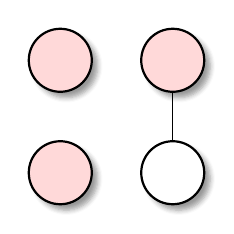
\begin{tikzpicture}[node distance=0.6cm]
  \node[activeN ] (a1) {};
  \node[activeN ] (a2) [above=of a1] {};
  \node[activeN ] (a3) [right=of a2] {};
  \node[passiveN] (a4) [below=of a3] {};
  \path
    (a3) edge (a4);
\end{tikzpicture}
\columnbreak

t = 4\\[10pt]
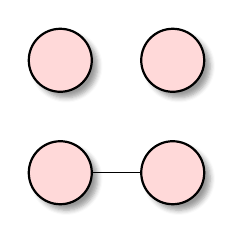
\begin{tikzpicture}[node distance=0.6cm]
  \node[activeN ] (a1) {};
  \node[activeN ] (a2) [above=of a1] {};
  \node[activeN ] (a3) [right=of a2] {};
  \node[activeN ] (a4) [below=of a3] {};
  \path
    (a4) edge (a1);
\end{tikzpicture}
\columnbreak

\color{white}{hallo}\\
\begin{mdframed}[linecolor=orange, leftmargin=-0.10cm,rightmargin=-0.2cm, roundcorner=10pt,innerbottommargin=10,innertopmargin=10,middlelinewidth=2]
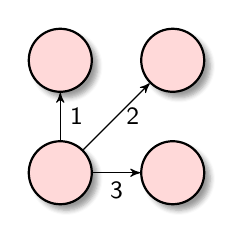
\begin{tikzpicture}[node distance=0.6cm]
  \node[activeN ] (a1) {};
  \node[activeN ] (a2) [above=of a1] {};
  \node[activeN ] (a3) [right=of a2] {};
  \node[activeN ] (a4) [below=of a3] {};
  \path[->]
    (a1) edge node [right] {1} (a2)
    (a1) edge node [right] {2} (a3)
    (a1) edge node [below] {3} (a4);
\end{tikzpicture}
\end{mdframed}
\end{multicols}
}

%=========================================================================================================================

\def\Zugangsmatrix{
\begin{multicols}{5}
\setlength{\columnseprule}{0.4pt}
\centering

Node $n_1$\\[10pt]
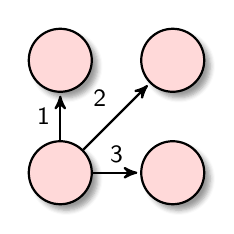
\begin{tikzpicture}[pil,node distance=0.6cm]
  \node[activeN ] (a1) {};
  \node[activeN ] (a2) [above=of a1] {};
  \node[activeN ] (a3) [right=of a2] {};
  \node[activeN ] (a4) [below=of a3] {};
  \path
    (a1) edge node {1} (a2)
    (a1) edge node {2} (a3)
    (a1) edge node {3} (a4);
\end{tikzpicture}
\columnbreak

Node $n_2$\\[10pt]
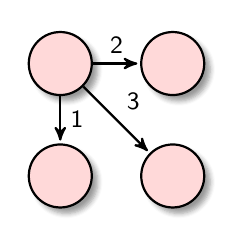
\begin{tikzpicture}[pil,node distance=0.6cm]
  \node[activeN ] (a1) {};
  \node[activeN ] (a2) [above=of a1] {};
  \node[activeN ] (a3) [right=of a2] {};
  \node[activeN ] (a4) [below=of a3] {};
  \path
    (a2) edge node {1} (a1)
    (a2) edge node {2} (a3)
    (a2) edge node {3} (a4);
\end{tikzpicture}
\columnbreak

Node $n_3$\\[10pt]
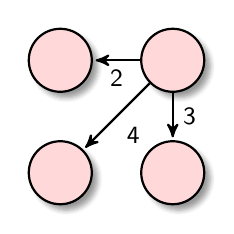
\begin{tikzpicture}[pil, node distance=0.6cm]
  \node[activeN ] (a1) {};
  \node[activeN ] (a2) [above=of a1] {};
  \node[activeN ] (a3) [right=of a2] {};
  \node[activeN ] (a4) [below=of a3] {};
  \path
    (a3) edge node {2} (a2)
    (a3) edge node {4} (a1)
    (a3) edge node {3} (a4);
\end{tikzpicture}
\columnbreak

Node $n_4$\\[10pt]
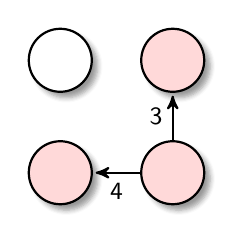
\begin{tikzpicture}[pil, node distance=0.6cm]
  \node[activeN ] (a1) {};
  \node[passiveN] (a2) [above=of a1] {};
  \node[activeN ] (a3) [right=of a2] {};
  \node[activeN ] (a4) [below=of a3] {};
  \path
    (a4) edge node {3} (a3)
    (a4) edge node {4} (a1);
\end{tikzpicture}
\columnbreak

$\mathcal{P}(T=4)$\\[2pt]
\begin{mdframed}[linecolor=orange, leftmargin=-0.10cm,rightmargin=-0.2cm, roundcorner=10pt,innerbottommargin=10,innertopmargin=10,middlelinewidth=2]
\centering
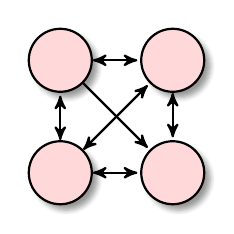
\begin{tikzpicture}[pil,node distance=0.6cm]
  \node[activeN ] (a1) {};
  \node[activeN ] (a2) [above=of a1] {};
  \node[activeN ] (a3) [right=of a2] {};
  \node[activeN ] (a4) [below=of a3] {};
  \path[<->]
    (a1) edge (a2)
    (a1) edge (a3)
    (a1) edge (a4)
    (a2) edge (a3)
    (a3) edge (a4);
  \path[->]
    (a2) edge (a4);
\end{tikzpicture}
\end{mdframed}
\end{multicols}
}

%=========================================================================================================================

\def\ZugangsmatrixNeu{
\begin{multicols}{5}
\setlength{\columnseprule}{0.4pt}
\centering

$G_I(t = 1)$\\[10pt]
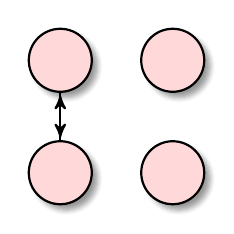
\begin{tikzpicture}[pil,node distance=0.6cm]
  \node[activeN ] (a1) {};
  \node[activeN ] (a2) [above=of a1] {};
  \node[activeN ] (a3) [right=of a2] {};
  \node[activeN ] (a4) [below=of a3] {};
  \path
    (a1) edge (a2)
    (a2) edge (a1);
\end{tikzpicture}
\columnbreak

$G_I(t = 2)$\\[10pt]
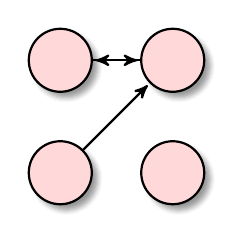
\begin{tikzpicture}[pil,node distance=0.6cm]
  \node[activeN ] (a1) {};
  \node[activeN ] (a2) [above=of a1] {};
  \node[activeN ] (a3) [right=of a2] {};
  \node[activeN ] (a4) [below=of a3] {};
  \path
    (a2) edge (a3)
    (a1) edge (a3)
    (a3) edge (a2);
\end{tikzpicture}
\columnbreak

$G_I(t = 3)$\\[10pt]
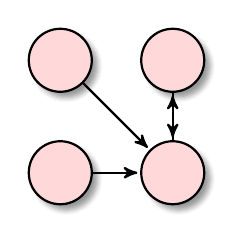
\begin{tikzpicture}[pil, node distance=0.6cm]
  \node[activeN ] (a1) {};
  \node[activeN ] (a2) [above=of a1] {};
  \node[activeN ] (a3) [right=of a2] {};
  \node[activeN ] (a4) [below=of a3] {};
  \path
    (a1) edge (a4)
    (a2) edge (a4)
    (a4) edge (a3)
    (a3) edge (a4);
\end{tikzpicture}
\columnbreak

$G_I(t = 4)$\\[10pt]
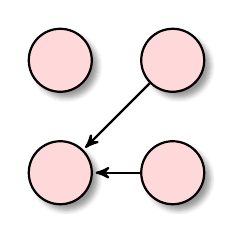
\begin{tikzpicture}[pil, node distance=0.6cm]
  \node[activeN ] (a1) {};
  \node[activeN ] (a2) [above=of a1] {};
  \node[activeN ] (a3) [right=of a2] {};
  \node[activeN ] (a4) [below=of a3] {};
  \path
    (a3) edge (a1)
    (a4) edge (a1);
\end{tikzpicture}
\columnbreak

$\mathcal{P}(T=4)$\\[2pt]
\begin{mdframed}[linecolor=orange, leftmargin=-0.10cm,rightmargin=-0.2cm, roundcorner=10pt,innerbottommargin=10,innertopmargin=10,middlelinewidth=2]
\centering
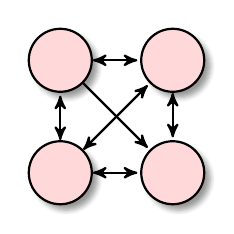
\begin{tikzpicture}[pil,node distance=0.6cm]
  \node[activeN ] (a1) {};
  \node[activeN ] (a2) [above=of a1] {};
  \node[activeN ] (a3) [right=of a2] {};
  \node[activeN ] (a4) [below=of a3] {};
  \path[<->]
    (a1) edge (a2)
    (a1) edge (a3)
    (a1) edge (a4)
    (a2) edge (a3)
    (a3) edge (a4);
  \path[->]
    (a2) edge (a4);
\end{tikzpicture}
\end{mdframed}
\end{multicols}
}

%=========================================================================================================================


\def\ZugangsmatrixSIR{
\begin{multicols}{5}
\setlength{\columnseprule}{0.4pt}
\centering

Node $n_1$\\[10pt]
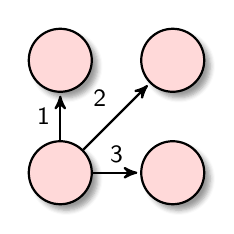
\begin{tikzpicture}[pil,node distance=0.6cm]
  \node[activeN ] (a1) {};
  \node[activeN ] (a2) [above=of a1] {};
  \node[activeN ] (a3) [right=of a2] {};
  \node[activeN ] (a4) [below=of a3] {};
  \path
    (a1) edge node {1} (a2)
    (a1) edge node {2} (a3)
    (a1) edge node {3} (a4);
\end{tikzpicture}
\columnbreak

Node $n_2$\\[10pt]
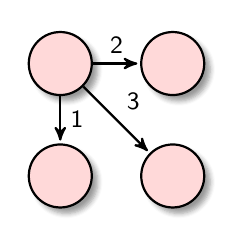
\begin{tikzpicture}[pil,node distance=0.6cm]
  \node[activeN ] (a1) {};
  \node[activeN ] (a2) [above=of a1] {};
  \node[activeN ] (a3) [right=of a2] {};
  \node[activeN ] (a4) [below=of a3] {};
  \path
    (a2) edge node {1} (a1)
    (a2) edge node {2} (a3)
    (a2) edge node {3} (a4);
\end{tikzpicture}
\columnbreak

Node $n_3$\\[10pt]
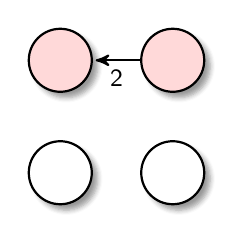
\begin{tikzpicture}[pil, node distance=0.6cm]
  \node[passiveN ] (a1) {};
  \node[activeN ] (a2) [above=of a1] {};
  \node[activeN ] (a3) [right=of a2] {};
  \node[passiveN ] (a4) [below=of a3] {};
  \path
    (a3) edge node {2} (a2);
\end{tikzpicture}
\columnbreak

Node $n_4$\\[10pt]
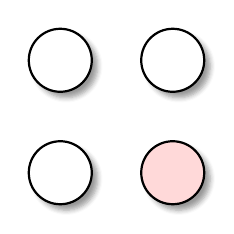
\begin{tikzpicture}[pil, node distance=0.6cm]
  \node[passiveN ] (a1) {};
  \node[passiveN] (a2) [above=of a1] {};
  \node[passiveN ] (a3) [right=of a2] {};
  \node[activeN ] (a4) [below=of a3] {};
\end{tikzpicture}
\columnbreak

$\mathcal{P}(T=4)$\\[2pt]
\begin{mdframed}[linecolor=orange, leftmargin=-0.10cm,rightmargin=-0.2cm, roundcorner=10pt,innerbottommargin=10,innertopmargin=10,middlelinewidth=2]
\centering
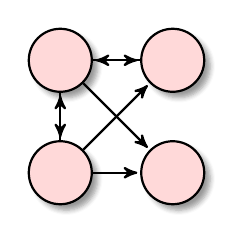
\begin{tikzpicture}[pil,node distance=0.6cm]
  \node[activeN ] (a1) {};
  \node[activeN ] (a2) [above=of a1] {};
  \node[activeN ] (a3) [right=of a2] {};
  \node[activeN ] (a4) [below=of a3] {};
  \path[->]
    (a1) edge (a2)
    (a1) edge (a3)
    (a1) edge (a4)
    (a2) edge (a1)
    (a2) edge (a3)
    (a2) edge (a4)
    (a3) edge (a2);
\end{tikzpicture}
\end{mdframed}
\end{multicols}
}
%-----------------------------------------------------------------------------------------------------------------------

\def\MatrixProduct{
\begin{multicols}{3}
%\setlength{\columnseprule}{0.4pt}

$A(T+1)$\\[10pt]
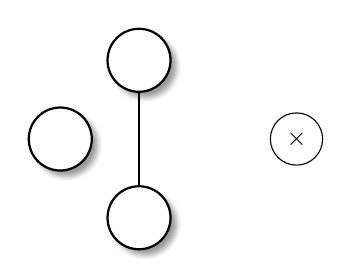
\begin{tikzpicture}[node distance=0.6cm]
  \node[passiveN ] (a1) at (0cm,0cm)		{};
  \node[passiveN ] (a2) at (1cm,1cm)	 	{};
  \node[passiveN ] (a3) at (1cm,-1cm)	 	{};
  \node[circle,draw=black,thin] (a4) at (3cm,0cm)	{$\times$};
  \path[thick]
    (a2) edge (a3);
\end{tikzpicture}
\columnbreak

\centering
$I(T)$\\[10pt]
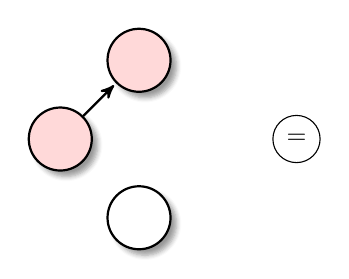
\begin{tikzpicture}[pil,node distance=0.6cm]
  \node[activeN  ] (a1) at (0cm,0cm)		{};
  \node[activeN  ] (a2) at (1cm,1cm)	 	{};
  \node[passiveN ] (a3) at (1cm,-1cm)	 	{};
  \node[circle,draw=black,thin] (a4) at (3cm,0cm)	{$=$};
  \path
    (a1) edge (a2);
\end{tikzpicture}
\columnbreak

$A(T+1) I(T)$\\[10pt]
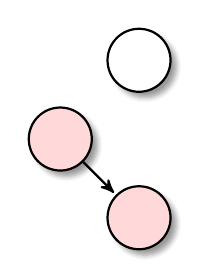
\begin{tikzpicture}[pil,node distance=0.6cm]
  \node[activeN ] (a1) at (0cm,0cm)		{};
  \node[passiveN] (a2) at (1cm,1cm)	 	{};
  \node[activeN ] (a3) at (1cm,-1cm)	 	{};
  \path
    (a1) edge (a3);
\end{tikzpicture}
\end{multicols}
}
%====================================================================================================================
\def\lesliescheme{

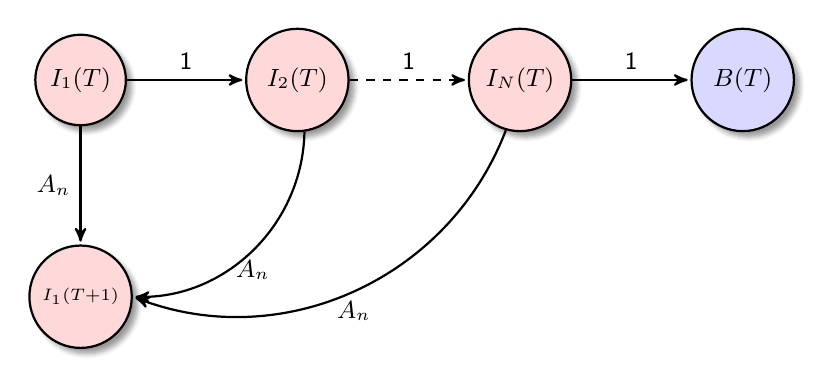
\begin{tikzpicture}[pil,node distance=1.5cm]
  \node[activeN] (I1) {$I_1(T)$};
  \node[activeN, minimum size=13mm] (I2) [right=of I1] {$I_2(T)$};
  \node[activeN, minimum size=13mm] (IN) [right=of I2] {$I_N(T)$};
  \node[activeN, fill=blue!15, minimum size=13mm] (R)  [right=of IN] {$B(T)$};
  \node[activeN, minimum size=13mm] (Ineu) [below=of I1] {$\scriptstyle I_1(T+1)$};
  \draw[dashed]
      (I2) edge node[above] {1} (IN);
  \draw
      (I1) edge node[above] {1} (I2)
      (IN) edge node[above] {1} (R)
      (I1) edge node[left] {$A_n$} (Ineu)
      (I2) edge[bend left=45] node[below] {$A_n$} (Ineu.east)
      (IN) edge[bend left=45] node[below] {$A_n$} (Ineu.east);
\end{tikzpicture}

}
%================================ figure ===============================================================================

\def\figurePopulationDynamics{

\begin{figure}[h]
\centering
\begin{subfigure}[t]{0.4\textwidth}
\centering
$
\begin{pmatrix}
 f_1 & f_2 & f_3 \\
 s_1 &  0  &  0  \\
  0  & s_2 &  0  \\
\end{pmatrix}
\cdot
\begin{pmatrix}
 a_1 \\
 a_2 \\
 a_3 \\
\end{pmatrix}
$
\caption{}
\label{pic:leslieM}
\end{subfigure}
%------------------------------------------------------------------------------------
\begin{subfigure}[t]{0.59\textwidth}
\centering
$
\underbrace{
\begin{pmatrix}
 \mathbf{A}(t) & \mathbf{A}(t) & \mathbf{A}(t) \\
 \mathbb{1} & \mathbb{0} & \mathbb{0} \\
 \mathbb{0} & \mathbb{1} & \mathbb{0} \\
\end{pmatrix}
}_{3 \cdot N}
\cdot
\left.
\begin{pmatrix}
  I_1 \\
  I_2 \\
  I_3 
\end{pmatrix}
\right\} 3 \cdot N
$
\caption{}
\label{pic:modifiedM}
\end{subfigure}
\caption{Figure~\ref{pic:leslieM} gives an example of a Leslie matrix with three age classes, each characterized by two parameters. The model can be compared to a modified SIS-type outbreak on temporal networks (fig.~\ref{pic:modifiedM}).}
\end{figure}
%=============================== end figure ========================================
}


%================================ figure =============================================
\def\tabularExample{
\renewcommand{\arraystretch}{1.1}
\begin{tabular}[H]{c|c|c}
 \bspEins & \bspZwei & \bspDrei \\ \hline
$
\begin{pmatrix}
 A(0) & A(0) & A(0) \\
 \mathbb{1} & \mathbb{0} & \mathbb{0} \\
 \mathbb{0} & \mathbb{1} & \mathbb{0} \\
\end{pmatrix}
\cdot
\begin{pmatrix}
 \vec{a}_1(0)\\
 \vec{a}_2(0)\\
 \vec{a}_3(0)\\
\end{pmatrix}
$
&
$
\begin{pmatrix}
 A(1) & A(1) & A(1) \\
 \mathbb{1} & \mathbb{0} & \mathbb{0} \\
 \mathbb{0} & \mathbb{1} & \mathbb{0} \\
\end{pmatrix}
\cdot
\begin{pmatrix}
 \vec{a}_1(1)\\
 \vec{a}_2(1)\\
 \vec{a}_3(1)\\
\end{pmatrix}
$
&
$
\begin{pmatrix}
 A(2) & A(2) & A(2) \\
 \mathbb{1} & \mathbb{0} & \mathbb{0} \\
 \mathbb{0} & \mathbb{1} & \mathbb{0} \\
\end{pmatrix}
\cdot
\begin{pmatrix}
 \vec{a}_1(2)\\
 \vec{a}_2(2)\\
 \vec{a}_3(2)\\
\end{pmatrix}
$ \\ \hline
$
A(0) = \begin{pmatrix}
        0 & 0 & 0 \\
	0 & 0 & 1 \\
	0 & 1 & 0 \\
       \end{pmatrix}
$ &
$
A(1) = \begin{pmatrix}
        0 & 0 & 0 \\
	0 & 1 & 0 \\
	1 & 0 & 0 \\
       \end{pmatrix}
$ &
$
A(2) = \begin{pmatrix}
        0 & 0 & 0 \\
	0 & 0 & 0 \\
	0 & 0 & 0 \\
       \end{pmatrix}
$
\\
$
\vec{a}_1(0) = \begin{pmatrix}
                1\\
                0\\
                0\\
               \end{pmatrix}
$ &
$
\vec{a}_1(1) = \begin{pmatrix}
                0\\
                0\\
                1\\
               \end{pmatrix}
$ &
$
\vec{a}_1(2) = \begin{pmatrix}
                1\\
                0\\
                0\\
               \end{pmatrix}
$ \\
$
\vec{a}_2(0) = \begin{pmatrix}
                0\\
                1\\
                0\\
               \end{pmatrix}
$ &
$
\vec{a}_2(1) = \begin{pmatrix}
                1\\
                0\\
                0\\
               \end{pmatrix}
$ &
$
\vec{a}_2(2) = \begin{pmatrix}
                0\\
                0\\
                1\\
               \end{pmatrix}
$ \\
$
\vec{a}_3(0) = \begin{pmatrix}
                0\\
                0\\
                0\\
               \end{pmatrix}
$ &
$
\vec{a}_3(1) = \begin{pmatrix}
                0\\
                1\\
                0\\
               \end{pmatrix}
$ &
$
\vec{a}_3(2) = \begin{pmatrix}
                1\\
                0\\
                0\\
               \end{pmatrix}
$ \\
\end{tabular}
}
%=============================== end figure ========================================

\def\tableSIRexample{

\setlength{\tabcolsep}{5mm}
%\renewcommand{\arraystretch}{2}
\begin{tabular}{c|c|c|c|c|c}
Zeit t & $A(t)$ & $I_1(t)$ & $I_2(t)$ & $R(t)$ & $\mathcal{P}(t)$\\[20pt] \hline
t = 0 & & $\begin{pmatrix}1 & 0 & 0 & 0 \\0 & 1 & 0 & 0 \\0 & 0 & 1 & 0 \\0 & 0 & 0 & 1\end{pmatrix}$ & $\begin{pmatrix}0 & 0 & 0 & 0 \\0 & 0 & 0 & 0 \\0 & 0 & 0 & 0 \\0 & 0 & 0 & 0\end{pmatrix}$ & $\begin{pmatrix}0 & 0 & 0 & 0 \\0 & 0 & 0 & 0 \\0 & 0 & 0 & 0 \\0 & 0 & 0 & 0\end{pmatrix}$ & $\begin{pmatrix}1 & 0 & 0 & 0 \\0 & 1 & 0 & 0 \\0 & 0 & 1 & 0 \\0 & 0 & 0 & 1\end{pmatrix}$\\[20pt] \hline
%
t = 1 & $\begin{pmatrix}0 & 1 & 0 & 0 \\1 & 0 & 0 & 0 \\0 & 0 & 0 & 0 \\0 & 0 & 0 & 0\end{pmatrix}$ & $\begin{pmatrix}0 & 1 & 0 & 0 \\1 & 0 & 0 & 0 \\0 & 0 & 0 & 0 \\0 & 0 & 0 & 0\end{pmatrix}$ & $\begin{pmatrix}1 & 0 & 0 & 0 \\0 & 1 & 0 & 0 \\0 & 0 & 1 & 0 \\0 & 0 & 0 & 1\end{pmatrix}$ & $\begin{pmatrix}0 & 0 & 0 & 0 \\0 & 0 & 0 & 0 \\0 & 0 & 0 & 0 \\0 & 0 & 0 & 0\end{pmatrix}$ & $\begin{pmatrix}1 & 1 & 0 & 0 \\1 & 1 & 0 & 0 \\0 & 0 & 1 & 0 \\0 & 0 & 0 & 1\end{pmatrix}$\\[20pt] \hline
%
t = 2 & $\begin{pmatrix}0 & 0 & 0 & 0 \\0 & 0 & 1 & 0 \\0 & 1 & 0 & 0 \\0 & 0 & 0 & 0\end{pmatrix}$ & $\begin{pmatrix}0 & 0 & 0 & 0 \\0 & 0 & 1 & 0 \\1 & 1 & 0 & 0 \\0 & 0 & 0 & 0\end{pmatrix}$ & $\begin{pmatrix}0 & 1 & 0 & 0 \\1 & 0 & 0 & 0 \\0 & 0 & 0 & 0 \\0 & 0 & 0 & 0\end{pmatrix}$ & $\begin{pmatrix}1 & 0 & 0 & 0 \\0 & 1 & 0 & 0 \\0 & 0 & 1 & 0 \\0 & 0 & 0 & 1\end{pmatrix}$ & $\begin{pmatrix}1 & 1 & 0 & 0 \\1 & 1 & 1 & 0 \\1 & 1 & 1 & 0 \\0 & 0 & 0 & 1\end{pmatrix}$\\[20pt] \hline
%
t = 3 & $\begin{pmatrix}0 & 0 & 0 & 0 \\0 & 0 & 0 & 0 \\0 & 0 & 0 & 1 \\0 & 0 & 1 & 0\end{pmatrix}$ & $\begin{pmatrix}0 & 0 & 0 & 0 \\0 & 0 & 0 & 0 \\0 & 0 & 0 & 0 \\1 & 1 & 0 & 0\end{pmatrix}$ & $\begin{pmatrix}0 & 0 & 0 & 0 \\0 & 0 & 1 & 0 \\1 & 1 & 0 & 0 \\0 & 0 & 0 & 0\end{pmatrix}$ & $\begin{pmatrix}1 & 1 & 0 & 0 \\1 & 1 & 0 & 0 \\0 & 0 & 1 & 0 \\0 & 0 & 0 & 1\end{pmatrix}$ & $\begin{pmatrix}1 & 1 & 0 & 0 \\1 & 1 & 1 & 0 \\1 & 1 & 1 & 0 \\1 & 1 & 0 & 1\end{pmatrix}$\\[20pt] \hline
%
t = 4 & $\begin{pmatrix}0 & 0 & 0 & 1 \\0 & 0 & 0 & 0 \\0 & 0 & 0 & 0 \\1 & 0 & 0 & 0\end{pmatrix}$ & $\begin{pmatrix}0 & 0 & 0 & 0 \\0 & 0 & 0 & 0 \\0 & 0 & 0 & 0 \\0 & 0 & 0 & 0\end{pmatrix}^*$ & $\begin{pmatrix}0 & 0 & 0 & 0 \\0 & 0 & 0 & 0 \\0 & 0 & 0 & 0 \\1 & 1 & 0 & 0\end{pmatrix}$ & $\begin{pmatrix}1 & 1 & 0 & 0 \\1 & 1 & 1 & 0 \\1 & 1 & 1 & 0 \\0 & 0 & 0 & 1\end{pmatrix}$ & $\begin{pmatrix}1 & 1 & 0 & 0 \\1 & 1 & 1 & 0 \\1 & 1 & 1 & 0 \\1 & 1 & 0 & 1\end{pmatrix}$\\
\end{tabular}

}


% ***********************************************************
% ********************** END HEADER *************************
% ***********************************************************